\chapter{性能测试}
\begin{table}[htbp]
\centering
\caption{实验环境}\label{tab:runconfig}
\begin{tabular}{l l}
\toprule
服务器 & Dell R730 \\
\midrule
操作系统 & Windows Server 2012 R2 \\
\midrule
CPU & Intel Xeon E5 2698 \\
\midrule
内存 & 128GB \\
\midrule
网卡 & Mellanox Connect-X 3 Pro \\
\midrule
FPGA & Altera Stratix V \\
\bottomrule
\end{tabular}
\end{table}
\begin{figure}[htbp]
\centering
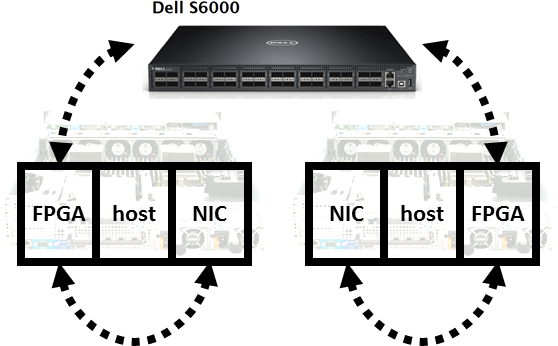
\includegraphics[width=4in]{connect}
\caption{网络拓扑}\label{fig:connect}
\end{figure}
我们在数据中心实验室服务器上评估RoCE的性能,其运行环境如表~\ref{tab:runconfig} 所示。
FPGA通过以太网端口与机架顶 (top-of-rack, ToR)的戴尔S6000交换机\cite{s6000}相连。
如图~\ref{fig:connect} 所示,主机通过网卡发出的RDMA包,经FPGA丢包及记录,由交换机到达接收端。

我们在主机上运行ndping、ndrping等程序,进行RDMA读、写、发送等数据操作,
测量其通信带宽及延迟,并与PCIe接口通信进行对比。

\begin{figure}[htbp]
\centering
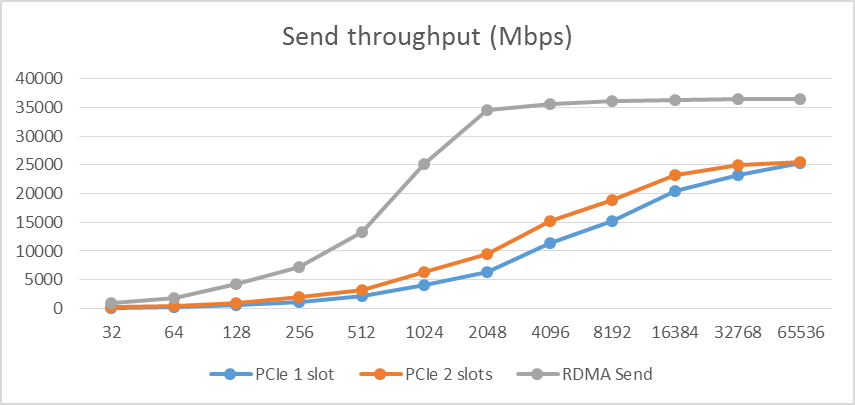
\includegraphics[width=4in]{rocerate}
\caption{RDMA Send与PCIe接口通信带宽对比}\label{fig:rocerate}
\note{横轴为对数坐标数据载荷大小 (字节), 纵轴为算术坐标通信带宽 (Gbps)\\实验中Send、Read、Write间性能差异在误差范围内,故只列出Send的数据}
\end{figure}

\begin{figure}[htbp]
\centering
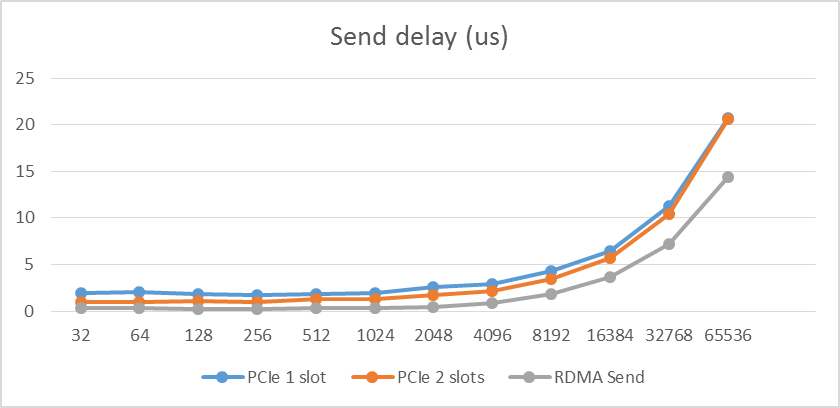
\includegraphics[width=4in]{rocelat}
\caption{RDMA Send与PCIe接口通信延迟对比}\label{fig:rocelat}
\note{横轴为对数坐标数据载荷大小 (字节), 纵轴为算术坐标通信延迟 (微秒)}
\end{figure}

\begin{figure}[htbp]
\centering
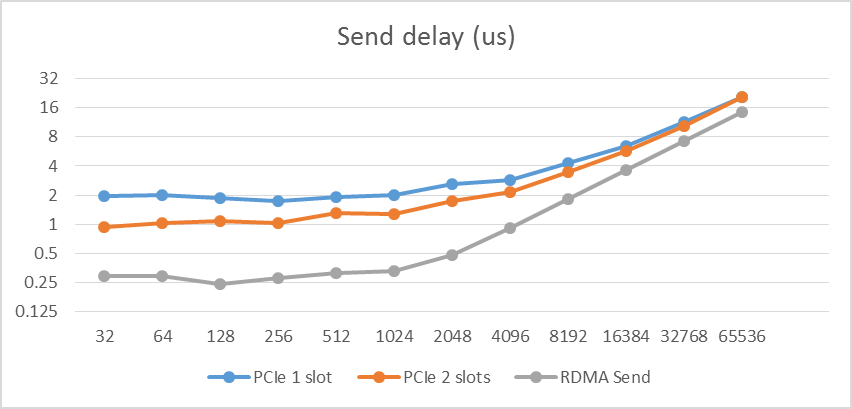
\includegraphics[width=4in]{rocelatlog}
\caption{RDMA Send与PCIe接口通信延迟对比(对数纵坐标)}\label{fig:rocelatlog}
\note{横轴为对数坐标数据载荷大小 (字节), 纵轴为对数坐标通信延迟 (微秒)}
\end{figure}

据图~\ref{fig:rocerate} 可见,随着数据载荷的增大,单位时间内需要处理的请求数目减少,
系统从计算密集向I/O密集转变,PCIe与RDMA均达到其带宽上限。
RDMA的通信带宽为40Gbps(实际中为36Gbps),高于PCIe接口的32Gbps(实际中25.6Gbps)。

据图~\ref{fig:rocelat}、图~\ref{fig:rocelatlog}可见,随着包的增大,帧数增多,
处理所需的周期数线性增加,在通信延迟上也得到了体现。

实验结果表明,RoCE能够有效利用网卡的通信带宽,实现比PCIe接口更高的传输速率以及更低的延迟。
使用RoCE替代PCIe通信能够提升FPGA的存储性能。
